%=======================================================
% CHAPTER 0: INTRODUCTION
%=======================================================

%--- Section Title Frame ---
\begin{frame}[plain]
  \begin{center}\bfseries\centering
    
\includegraphics[scale=1]{assets/branding/opa0}
    \vspace{-5.75cm}\\
    {\adjustbox{scale=2.5}{\color{TealDarkCyan}\;I.\;Introduction}}
    \bigskip\bigskip
    {\ }\vspace{4cm}\\
    \bigskip
  \end{center}
\end{frame}

%--- Slide: Errors Are Everywhere ---
\begin{frame}[fragile]{\textbf{I. Introduction}}{Errors Are Everywhere}\small
\begin{columns}[T,onlytextwidth]
\begin{column}{.68\textwidth}
    \textcolor{TealDarkCyan}{\textbf{Physical world}}
    \begin{itemize}
      \item Scratches on a CD or DVD
    \end{itemize}
    \bigskip
    \textcolor{TealDarkCyan}{\textbf{Digital world}}
    \begin{itemize}
      \item Bit flips during internet transmission
    \end{itemize}
  \end{column}
  \begin{column}{.3\textwidth}
  	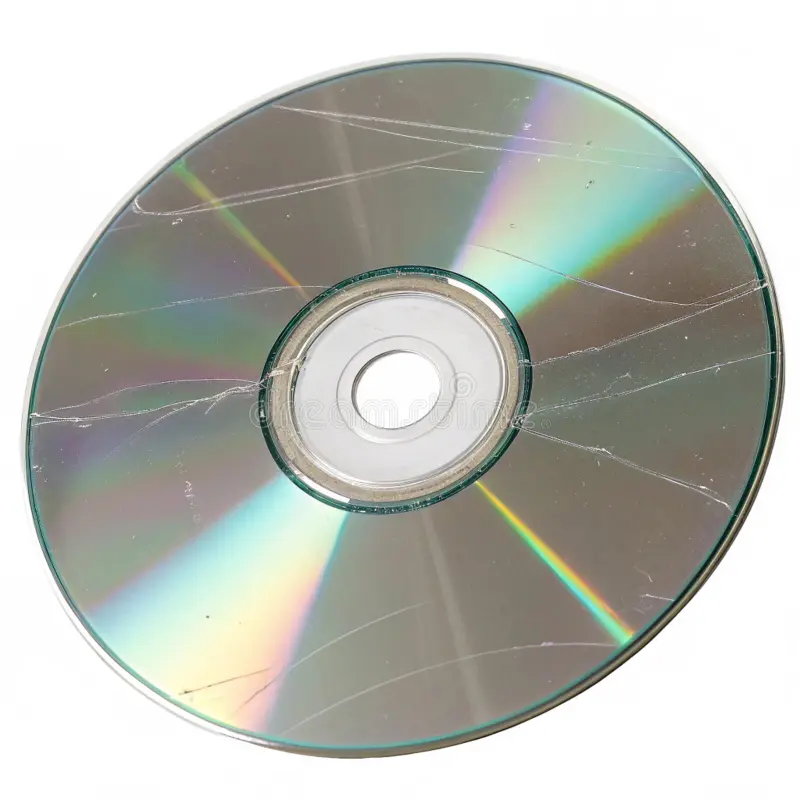
\includegraphics[scale=.1]{assets/image/scratched-cd}
\end{column}
\end{columns}
\vfill
\textbf{\color{red}Questions.} \begin{center}
	``How do we transmit (or store) data \textbf{reliably} in the presence of noise?''
\end{center}
\end{frame}

%--- Slide: Can We Make Noisy Data Reliable Again? ---
\begin{frame}[fragile]{\textbf{I. Introduction}}{Can We Make Noisy Data Reliable Again?}\small
\begin{center}
\begin{tikzpicture}[scale=0.92]
	% A simple "bit flip" picture
	\node[font=\ttfamily\large] at (0,3.0) {%
  $\cdots$1\,1\,1\,1\,0\,1\,1\,0\,1\,0\,1\,0\,1\,1\,0\,0\,1$\cdots$};
	\draw[-Stealth, thick, AccentCyan!70!black, dashed]
	(0,2.55) -- node[right=2pt,font=\footnotesize]{noise} (0,1.85);
	\node[font=\ttfamily\large] at (0,1.5) {%
  $\cdots$1\,1\,1\,1\,0\,1\,1\,0\,1\,0\,1\,0\,\textcolor{red!70!black}{0}\,1\,0\,0\,1$\cdots$};
\end{tikzpicture}
\end{center}
\bigskip
\begin{itemize}
	\item<2-> Can we \textbf{detect} it?
	\item[]
	\item<3-> Can we \textbf{fix} it?
\end{itemize}
\end{frame}

%%--- Slide: Familiar Example 1 — Check Digits ---
%\begin{frame}{\textbf{I. Introduction}}{A Familiar Example: Check Digits}
%\small
%Every ISBN-10 (International Standard Book Number) ends with a \textbf{check digit}.
%
%\medskip
%
%\textbf{Example.}\; ISBN $0\text{-}306\text{-}40615\text{-}2$: \begin{align*}
%&\; 1{\cdot}0 + 2{\cdot}3 + 3{\cdot}0 + 4{\cdot}6 + 5{\cdot}4 +\; 6{\cdot}0 + 7{\cdot}6 + 8{\cdot}1 + 9{\cdot}5 + 10{\cdot}2 \\
%=&\; 0+6+0+24+20+0+42+8+45+20 \\[2pt]
%=&\; 165 \;=\; 15\times11. \;\checkmark
%\end{align*}
%%\defbox[ISBN-10 check condition]{
%%For digits $d_1d_2\cdots d_{10}$ (where $d_{10}\in\{0,1,\ldots,9,X\}$, $X=10$), \[
%%  \sum_{i=1}^{10} i\cdot d_i \;\equiv\; 0 \pmod{11}.
%%\]}
%\textcolor{TealDarkCyan}{\textbf{What it guarantees}}
%\begin{itemize}
%	\item Detects \emph{every} single-digit error
%	\item Detects \emph{every} transposition of two adjacent digits
%\end{itemize}
%\bigskip
%\textcolor{AccentCyan!80!black}{\textbf{Limitation}}
%\begin{itemize}
%	\item One check digit $\Rightarrow$ detects errors, cannot \emph{correct} them
%\end{itemize}
%\end{frame}

%--- Slide: Repetition ---
\begin{frame}{\textbf{I. Introduction}}{Triple Repetition Code $\nkcode{3}{1}{2}$}
\small
The simplest way to correct errors: \textbf{say it three times}. \[
  \texttt{0} \;\longmapsto\; \texttt{000}, \qquad \texttt{1} \;\longmapsto\; \texttt{111}.
\]
%\medskip
%\defbox[Triple repetition code]{
%Encode one bit by repeating it three times:
%\[
%  0 \;\longmapsto\; 000, \qquad 1 \;\longmapsto\; 111.
%\]%\textbf{Decoding rule (majority vote):} decide the bit that appears most often.
%}
\begin{center}
\begin{minipage}{.49\textwidth}\centering
\begin{tabular}{c|c|c}
	\textbf{Received} & \textbf{Majority} & \textbf{Decision} \\\hline
	\rowcolor{TealDarkCyan!8} $\texttt{000}$ & $\texttt{0} \times 3$ & $\texttt{0}$ \\
	$\texttt{001}$ & $\texttt{0} \times 2$ & $\texttt{0}$ \\
	\rowcolor{TealDarkCyan!8} $\texttt{010}$ & $\texttt{0} \times 2$ & $\texttt{0}$ \\
	$\texttt{100}$ & $\texttt{0} \times 2$ & $\texttt{0}$ \\
	\rowcolor{AccentCyan!10} $\texttt{011}$ & $\texttt{1} \times 2$ & $\texttt{1}$ \\
	$\texttt{101}$ & $\texttt{1} \times 2$ & $\texttt{1}$ \\
	\rowcolor{AccentCyan!10} $\texttt{110}$ & $\texttt{1} \times 2$ & $\texttt{1}$ \\
	$\texttt{111}$ & $\texttt{1} \times 3$ & $\texttt{1}$ \\
\end{tabular}
\end{minipage}
\begin{minipage}{.49\textwidth}\centering
\begin{tikzpicture}[scale=0.92, font=\scriptsize]
	\node[circle,draw=TealDarkCyan,fill=TealDarkCyan!22,minimum size=.56cm] (c0) at (0,0) {$\texttt{000}$};
	\node[circle,draw=TealDarkCyan,fill=AccentCyan!20,minimum size=.56cm] (c1) at (3,0) {$\texttt{111}$};
	
	\draw[TealDarkCyan!60,thick,dashed] (c0) circle (1cm);
	\draw[AccentCyan!60,thick,dashed] (c1) circle (1cm);
	
	\node[circle,draw=black,fill=white,minimum size=.56cm] (r1) at (0,1) {$\texttt{100}$};
	\node[circle,draw=black,fill=white,minimum size=.56cm] (r2) at (-1,0) {$\texttt{010}$};
	\node[circle,draw=black,fill=white,minimum size=.56cm] (r3) at (0,-1) {$\texttt{001}$};
	\node[circle,draw=black,fill=red!12,minimum size=.56cm] (w110) at (2,0) {$\texttt{110}$};
	
	\draw[black!50, thin] (c0) -- (r1) node[midway,right, font=\tiny]{$1$};
	\draw[black!50, thin] (c0) -- (r2) node[midway,above, font=\tiny]{$1$};
	\draw[black!50, thin] (c0) -- (r3) node[midway,right, font=\tiny]{$1$};
	\draw[red!60!black, thick] (c0) -- (w110) node[midway, above, font=\tiny]{$2$};
	\draw[red!60!black, thick] (w110) -- (c1) node[midway, above, font=\tiny]{$1$};
	
%	\node[font=\tiny] at (1.5,-1.75) {\textbf{2-bit flips from \(000\): \(110,101,011\notin\{000,111\}\)}};
%	\node[font=\tiny,TealDarkCyan] at (1.5,-2) {\textbf{$001,101,011,110\notin C\Rightarrow$ detected (not a codeword)}};
%	\node[font=\tiny,red!70!black] at (1.5,-2.25) {\textbf{$110$ is decoded to $111$}};
	
	\node[font=\tiny,TealDarkCyan!80!black,align=center] at (1.5,-1.75)
	{\textbf{2-bit errors are detectable, but not always correctable.}};
\end{tikzpicture}
\end{minipage}
\end{center}
\begin{columns}[T,onlytextwidth]
\begin{column}{.375\textwidth}
\textcolor{TealDarkCyan}{\textbf{Performance}}
\begin{itemize}
	\item Detects any two-bit flips
	\item Corrects any single-bit flip
\end{itemize}
\end{column}
\begin{column}{.55\textwidth}
\textcolor{AccentCyan!80!black}{\textbf{Cost}}
\begin{itemize}
	\item Rate $R = 1/3$: send $3$ bits to convey $1$ bit
	\item Very inefficient!
\end{itemize}
\end{column}
\end{columns}
\vfill
\textbf{\color{red}Question.}\; Can we do much better?
\end{frame}

%--- Slide: Distance Intuition ---
\begin{frame}{\textbf{I. Introduction}}{The Key Idea: Distance}
\small
Why does the triple repetition code work? The two codewords are \textbf{far apart}.

\medskip
\begin{center}
\begin{minipage}{.49\textwidth}\centering
\begin{tikzpicture}[scale=0.95]
	% 3-cube nodes — explicit (no \foreach with color params to avoid xcolor whitespace bug)
	\node[circle,draw=TealDarkCyan,fill=TealDarkCyan!20,minimum size=.56cm,font=\scriptsize,inner sep=1pt] (v000) at (0.0, 0.0) {$000$};
	\node[circle,draw=TealDarkCyan,fill=white,           minimum size=.56cm,font=\scriptsize,inner sep=1pt] (v100) at (2.0, 0.0) {$100$};
	\node[circle,draw=TealDarkCyan,fill=white,           minimum size=.56cm,font=\scriptsize,inner sep=1pt] (v010) at (1.0, 0.9) {$010$};
	\node[circle,draw=TealDarkCyan,fill=white,           minimum size=.56cm,font=\scriptsize,inner sep=1pt] (v110) at (3.0, 0.9) {$110$};
	\node[circle,draw=TealDarkCyan,fill=white,           minimum size=.56cm,font=\scriptsize,inner sep=1pt] (v001) at (0.5, 1.6) {$001$};
	\node[circle,draw=TealDarkCyan,fill=white,           minimum size=.56cm,font=\scriptsize,inner sep=1pt] (v101) at (2.5, 1.6) {$101$};
	\node[circle,draw=TealDarkCyan,fill=white,           minimum size=.56cm,font=\scriptsize,inner sep=1pt] (v011) at (1.5, 2.5) {$011$};
	\node[circle,draw=TealDarkCyan,fill=TealDarkCyan!20,minimum size=.56cm,font=\scriptsize,inner sep=1pt] (v111) at (3.5, 2.5) {$111$};
	% Edges
	\foreach \a/\b in {v000/v001,v111/v011,v111/v101,v001/v011,v001/v101,v101/v100,v110/v110}
	\draw[TealDarkCyan!40] (\a)--(\b);
	\foreach \a/\b in {v000/v100,v111/v110,v100/v110}
	\draw[red] (\a)--(\b);
	\foreach \a/\b in {v000/v010,v010/v110,v010/v011}
	\draw[TealDarkCyan!40,dashed] (\a)--(\b);
	% Labels
	\node[above=2pt of v000,font=\scriptsize,TealDarkCyan]{\textbf{codeword}};
	\node[above=2pt of v111,font=\scriptsize,TealDarkCyan]{\textbf{codeword}};
\end{tikzpicture}
\end{minipage}\hfill
\begin{minipage}{.49\textwidth}
\begin{tikzpicture}[scale=0.92, font=\scriptsize]
	\tikzset{
		bitnode/.style={circle,draw=TealDarkCyan,minimum size=.56cm,fill=white},
		codeword/.style={circle,draw=TealDarkCyan,minimum size=.68cm,fill=TealDarkCyan!18}
	}
	%\draw[TealDarkCyan!40, very thick] (0,0.75) ellipse (4cm and 2.25cm);
	\node[codeword] (v000) at (-1.5,0.45) {\(000\)};
	\node[codeword] (v111) at (1.5,0.45) {\(111\)};
	
	\draw[TealDarkCyan!75, very thick, dashed] (v000) circle (1cm);
	\draw[TealDarkCyan!75, very thick, dashed] (v111) circle (1cm);
	
	\node[bitnode] (v001) at (-2.5,.45) {\(001\)};
	\node[bitnode] (v010) at (-1.5,1.45) {\(010\)};
	\node[bitnode] (v100) at (-1.5,-0.5) {\(100\)};
	
	\node[bitnode] (v110) at (1.5,-0.5) {\(110\)};
	\node[bitnode] (v101) at (1.5,1.45) {\(101\)};
	\node[bitnode] (v011) at (2.5,.45) {\(011\)};
	
	\draw[green!60!black,-Latex] (v001) -- (v000);
	\draw[green!60!black,-Latex] (v010) -- (v000);
	\draw[green!60!black,-Latex] (v100) -- (v000);
	\draw[green!60!black,-Latex] (v110) -- (v111);
	\draw[green!60!black,-Latex] (v101) -- (v111);
	\draw[green!60!black,-Latex] (v011) -- (v111);
	
	\node[font=\tiny,green!70!black,align=center,text width=2.8cm] at (-1.5,2.25)
	{\textbf{1-bit errors\\correct to \(000\)}};
	\node[font=\tiny,green!70!black,align=center,text width=2.8cm] at (1.5,2.25)
	{\textbf{1-bit errors\\correct to \(111\)}};
	\draw[red,Latex-Latex] (v000) -- (v111) node[midway,above] {$3$};
\end{tikzpicture}
\end{minipage}
\end{center}
\vfill
\defbox[Minimum distance]{
A code with minimum distance $d$ corrects all errors of weight $\displaystyle\le\left\lfloor\frac{(d-1)}{2}\right\rfloor$.
}
\end{frame}


%--- Slide: Distance Meaning I ---
\begin{frame}{\textbf{I. Introduction}}{Hamming Distance}
\small
Hamming distance counts how many coordinates differ. For any $\mathbf{x},\mathbf{y}\in\F_2^n$, \[
  d_H(\mathbf{x},\mathbf{y})=
  w_H(\mathbf{x}\oplus\mathbf{y})=\#\{i:\ x_i\neq y_i\}
\] where \(w_H\) is Hamming weight (number of ones).
\medskip

\begin{center}
\begin{tikzpicture}[scale=0.95]
	% Two strings with differences highlighted
	\foreach \i/\a/\b in {1/1/1, 2/0/1, 3/1/0, 4/1/1, 5/0/0, 6/0/1, 7/1/1} {
		\pgfmathsetmacro{\xpos}{(\i-1)*0.9}
		\ifnum\a=\b
		\node[minimum size=0.75cm, draw=TealDarkCyan!40, rounded corners=3pt,
		fill=TealDarkCyan!8, font=\small] at (\xpos, 0.6) {$\a$};
		\node[minimum size=0.75cm, draw=TealDarkCyan!40, rounded corners=3pt,
		fill=TealDarkCyan!8, font=\small] at (\xpos,-0.6) {$\b$};
		\else
		\node[minimum size=0.75cm, draw=AccentCyan, thick, rounded corners=3pt,
		fill=AccentCyan!18, font=\small\bfseries] at (\xpos, 0.6) {$\a$};
		\node[minimum size=0.75cm, draw=AccentCyan, thick, rounded corners=3pt,
		fill=AccentCyan!18, font=\small\bfseries] at (\xpos,-0.6) {$\b$};
		\draw[AccentCyan, thick, <->] (\xpos,0.22) -- (\xpos,-0.22)
		node[midway,right=1pt,font=\tiny]{$\neq$};
		\fi
	}
	\node[left=4pt, font=\small] at (-0.4, 0.6) {$x=$};
	\node[left=4pt, font=\small] at (-0.4,-0.6) {$y=$};
	\node[right=4pt, font=\small, TealDarkCyan] at (6, 0) {$d(x,y)=3$};
\end{tikzpicture}
\end{center}

\noindent
\textbf{Example 1.}\; \(d_H(0101,1100)=2\).
\medskip

\textbf{Example 2.}\; \(d_H(000,101)=2\).

\vfill

\textcolor{TealDarkCyan}{\textbf{Hamming distance is a metric}.} 
%\begin{enumerate}[(i)]
%	\item $d_H(\mathbf{x},\mathbf{y})\ge 0,
%	\ d_H(\mathbf{x},\mathbf{y})=0 \iff \mathbf{x}=\mathbf{y},$
%	\item $  d_H(\mathbf{x},\mathbf{y}) = d_H(\mathbf{y},\mathbf{x}),$
%	\item $d_H(\mathbf{x},\mathbf{z}) \le d_H(\mathbf{x},\mathbf{y}) + d_H(\mathbf{y},\mathbf{z}).$
%\end{enumerate}
\end{frame}

%--- Slide: Correction Balls ---
\begin{frame}{\textbf{I. Introduction}}{Correction Balls}
\small
\begin{center}
\begin{tikzpicture}[scale=0.95, font=\scriptsize]
\tikzset{
	cnode/.style={circle,draw=TealDarkCyan,fill=TealDarkCyan!18,minimum size=.64cm,very thick},
	grid/.style={line width=.6pt}
}
\foreach \i/\x/\y/\L in {
	1/-4/ 1.5/{$c_1$},
	2/-3/ -2/{$c_2$},
	3/0/ 0/{$c_3$},
	4/3/ 1.70/{$c_4$},
	5/4/-1.25/{$c_5$}
}{
	\node[cnode] (c\i) at (\x,\y) {\L};
}
\node[cnode, draw=red, fill=red!20] at (1,1) {};
\node[cnode, draw=red, fill=red!20] at (2,-1) {};
\node[cnode, draw=red, fill=red!20] at (-1.75,-.5) {};
\node[cnode, draw=red, fill=red!20] at (-2.75,.5) {};
\node[cnode, draw=red, fill=red!20] at (2,1.25) {};
\only<2>{\foreach \i in {1,...,5} {\draw[TealDarkCyan,dashed, thick] (c\i) circle (1cm);}}
\only<3>{\foreach \i in {1,...,5} {\draw[TealDarkCyan,dashed, very thick] (c\i) circle (1.5cm);}}
\only<4>{\foreach \i in {1,...,5} {\draw[Red!70!black,dashed, very thick] (c\i) circle (1.75cm);}}
\end{tikzpicture}
\end{center}
\only<4>{\textbf{Remark.}\; \textcolor{TealDarkCyan}{\textbf{No overlap of correction balls} $\;\Longleftrightarrow\;$ unique decoding is possible.}}
\end{frame}

%%--- Slide: QR Codes ---
%\begin{frame}{\textbf{I. Introduction}}{Real-World Example: QR Codes}
%\small
%\begin{columns}[T,onlytextwidth]
%  \begin{column}{.54\textwidth}
%    QR codes use \textbf{Reed--Solomon error correction} — a powerful algebraic code.
%
%    \bigskip
%    \defbox[Four error-correction levels]{
%    \begin{tabular}{c|l|l}
%      \textbf{Level} & \textbf{Recovery} & \textbf{Use case} \\\hline
%      L & up to $7\%$ & clean environments\\
%      M & up to $15\%$ & standard use\\
%      Q & up to $25\%$ & industrial\\
%      H & up to $30\%$ & high damage risk
%    \end{tabular}
%    }
%
%    \bigskip
%    \textcolor{TealDarkCyan}{\textbf{Why Reed--Solomon?}}
%    \begin{itemize}
%      \item Designed for \emph{burst errors} (adjacent damage)
%      \item Algebraic structure enables fast decoding
%      \item Same code used in CDs, DVDs, Blu-ray
%    \end{itemize}
%  \end{column}
%  \begin{column}{.43\textwidth}
%    \begin{center}
%    \begin{tikzpicture}[scale=0.85]
%      % Draw a schematic QR-code grid
%      \foreach \x in {0,...,6}
%        \foreach \y in {0,...,6}
%          \fill[TealDarkCyan!15] (\x*0.35, \y*0.35) rectangle ++(0.32,0.32);
%      % Finder patterns (top-left)
%      \fill[TealDarkCyan]    (0,6*0.35) rectangle ++(7*0.35,0.35);
%      \fill[TealDarkCyan]    (0,0) rectangle ++(7*0.35,0.35);
%      \fill[TealDarkCyan]    (0,0) rectangle ++(0.35,7*0.35);
%      \fill[TealDarkCyan]    (6*0.35,0) rectangle ++(0.35,7*0.35);
%      \fill[white]           (0.35,0.35) rectangle ++(5*0.35,5*0.35);
%      \fill[TealDarkCyan]    (0.7,0.7) rectangle ++(3*0.35,3*0.35);
%      % A "damage" patch
%      \fill[AccentCyan!35]   (1.2,1.15) rectangle ++(0.9,0.9);
%      \node[font=\tiny, AccentCyan!80!black] at (1.65,1.6) {damage};
%      % Label
%      \node[font=\footnotesize, TealDarkCyan] at (1.225,-0.3)
%        {still readable!};
%    \end{tikzpicture}
%    \end{center}
%    \bigskip
%    \begin{block}{}
%    \centering\small
%    Up to $30\%$ of a QR code can be destroyed and it still decodes correctly.
%    \end{block}
%  \end{column}
%\end{columns}
%\end{frame}

%--- Slide: The Communication Problem ---
\begin{frame}{\textbf{I. Introduction}}{The Communication Model}
\begin{center}
\begin{tikzpicture}[
>=Stealth,
block/.style={
	draw=TealDarkCyan, thick, fill=AccentCyan!80!black, rounded corners=2mm,
	minimum width=1.2cm, minimum height=1cm, align=center,
	font=\sffamily, drop shadow={opacity=0.15, shadow xshift=1mm, shadow yshift=-1mm}
},
adder/.style={
	circle, draw=TealDarkCyan, thick, fill=AccentCyan!80!black,
	minimum size=6mm, inner sep=0pt, align=center, font=\Large,
	drop shadow={opacity=0.15, shadow xshift=1mm, shadow yshift=-1mm}
},
arrow/.style={->, thick, TealDarkCyan},
mathlabel/.style={font=\normalsize, text=black},
sublabel/.style={font=\small\sffamily, text=magenta},
scale=.75
]

% Invisible nodes to act as the start and end points of the signals
\node (start) at (0,0) {};
\node (end)   at (19,0) {};

% Main operational blocks
\node[block, align=center, font=\color{white}] (enc) at (4.5,0) {Encoder\\ $\F_2^k\to\F_2^n$};
\onslide<2->\node[adder, font=\color{white}] (add) at (9.5,0) {$+$};
\onslide<3->\node[block, align=center, font=\color{white}] (dec) at (14.5,0) {Decoder\\ $\F_2^n\to\F_2^k$};

% Noise entry point
\onslide<2->\node (noise) at (9.5, 2) {\small \texttt{Noise} $\vect{e}$};

% --- Signal Paths & Labels ---

% Source to Encoder
\onslide<1->\draw[arrow] (start) -- 
node[midway, mathlabel, draw=TealDarkCyan, fill=white, align=center] {\texttt{message}\\ [-1.25mm] $\vect{x}$} node[below=5mm, sublabel] {$k$-bit} (enc);

% Encoder to Channel (Adder)
% We use a standard label below the arrow to replace the underbrace in the equation
\onslide<1->\draw[arrow] (enc) -- 
node[midway, mathlabel, draw=TealDarkCyan, fill=white, align=center] {\texttt{codeword}\\ [-1.25mm] $\vect{c}$} node[below=5mm, sublabel] {$n$-bit ($n>k$)} (add);

% Noise entering the Channel
\onslide<2->\draw[arrow] (noise) -- (add);

% Channel to Decoder
\onslide<2->\draw[arrow] (add) -- 
node[midway, mathlabel, draw=TealDarkCyan, fill=white, align=center] {\texttt{received}\\ [-1.25mm]  \texttt{vector} $\vect{y}$} node[below=5mm, sublabel] {$n$-bit} (dec);

% Decoder to Destination
\onslide<3->\draw[arrow] (dec) -- 
node[midway, mathlabel, draw=TealDarkCyan, fill=white, align=center] {\texttt{message}\\ [-1.25mm] $\widehat{\vect{x}}$} node[below=5mm, sublabel] {$k$-bit} (end);

\onslide<2->\draw[dashed, red] (8.7,-1.2) rectangle (10.3,2.5);
\onslide<2->\node[red] at (9.5,3) {channel};
\end{tikzpicture}
\end{center}
%\begin{center}
%\begin{tikzpicture}[
%  cbox/.style   = {draw, thick, rounded corners=4pt, minimum height=.85cm,
%                   minimum width=1.8cm, align=center},
%  arr/.style    = {-Stealth, thick, color=TealDarkCyan},
%  noise/.style  = {-Stealth, thick, color=AccentCyan!80!black},
%  lbl/.style    = {font=\small}
%]
%  \node[cbox, fill=TealDarkCyan!15] (src) {\small Source\\[-2pt]$\mathbf{m}$};
%  \node[cbox, fill=TealDarkCyan!25, right=1.1cm of src]  (enc) {\small Encoder};
%  \node[cbox, fill=AccentCyan!18,    right=1.1cm of enc]  (ch)  {\small Noisy\\[-2pt]\small Channel};
%  \node[cbox, fill=TealDarkCyan!25, right=1.1cm of ch]   (dec) {\small Decoder};
%  \node[cbox, fill=TealDarkCyan!15, right=1.1cm of dec]  (dst) {\small Receiver\\[-2pt]$\hat{\mathbf{m}}$};
%  \node[above=.55cm of ch, AccentCyan!80!black]    (err) {\small $\mathbf{e}$\; (noise)};
%
%  \draw[arr] (src) -- (enc) node[midway,above,lbl]{$\mathbf{m}$};
%  \draw[arr] (enc) -- (ch)  node[midway,above,lbl]{$\mathbf{c}$};
%  \draw[arr] (ch)  -- (dec) node[midway,above,lbl]{$\mathbf{v}=\mathbf{c}+\mathbf{e}$};
%  \draw[arr] (dec) -- (dst) node[midway,above,lbl]{$\hat{\mathbf{m}}$};
%  \draw[noise] (err) -- (ch);
%\end{tikzpicture}
%\end{center}
\bigskip
\begin{columns}[T,onlytextwidth]
\begin{column}{.4\textwidth}
\textbf{Setup}
\begin{itemize}\small
	\item Message $\mathbf{x}\in\F_q^k$
	\item Encoder : $\mathbf{x}\mapsto\mathbf{c}\in\F_q^n$,\; $n>k$
	\item Channel : $\mathbf{y}=\mathbf{c}\oplus\mathbf{e}$
\end{itemize}
\end{column}
\begin{column}{.58\textwidth}
\textbf{Goal}
	\begin{itemize}\small
	\item Recover $\hat{\mathbf{x}}=\mathbf{x}$ even when $\mathbf{e}\neq\mathbf{0}$
	\item Keep rate $R = k/n$ as large as possible
	\end{itemize}
\end{column}
\end{columns}
\end{frame}

%--- Slide: The Rate--Distance Tradeoff ---
\begin{frame}{\textbf{I. Introduction}}{The Fundamental Tradeoff}\small
\begin{center}\renewcommand{\arraystretch}{1.25}
\begin{tabular}{l|ccc}
	\textbf{Code} & \textbf{Rate} & \textbf{Detects} & \textbf{Corrects} $t$\\\hline
	$\nkdcode{n}{k}{d}{q}$-code & $k/n$&  $d-1$ & $\left\lfloor(d-1)/2\right\rfloor$\\\hline
	Repetition $\nkdcode{3}{1}{3}{2}$ & $1/3\approx0.33$ & 2 & 1 \\
	Hamming $[7,4,3]_2$ & $4/7\approx 0.57$ & 2 & 1 \\
	BCH $[15,7,5]_2$ & $7/15\approx 0.47$ & 4 & 2 \\
	Reed-Solomon $[15,11,5]_{16}$ & $11/15\approx 0.73$ & 4 & 2 \\
	Reed-Solomon $[255,223,33]_{256}$ & $223/255\approx 0.87$ & 32 & 16 \\
\end{tabular}
\end{center}
\begin{itemize}
	\item high rate $\implies$ efficiency
	\item correct many errors $\implies$ powerful
\end{itemize}
%\vspace{-2pt}
%\begin{center}
%\begin{tikzpicture}[x=7.6cm, y=1.25cm, font=\scriptsize]
%	% light grid
%	\draw[thin,gray!22] (0,0) grid[xstep=0.2,ystep=1] (1.0,2.7);
%	% axes
%	\draw[-Stealth,thick,TealDarkCyan] (-0.018,0) -- (1.10,0)
%	node[right,font=\small]{Rate $R=k/n$};
%	\draw[-Stealth,thick,TealDarkCyan] (0,-0.18) -- (0,3.05)
%	node[above,font=\small]{Correctable errors $t$};
%	% x ticks
%	\foreach \x in {0.2,0.4,0.6,0.8,1.0}
%	\draw[gray!60] (\x,0)--++(0,-0.12)
%	  node[below=1pt,font=\tiny]{\pgfmathprintnumber[fixed,precision=1]{\x}};
%	% y ticks
%	\foreach \y in {1,2}
%	\draw[gray!60] (0,\y)--++(-0.016,0) node[left=1pt,font=\tiny]{$\y$};
%%	% Singleton bound for n=15: t = 7.5(1-R)
%%	% enters plot at R=1-2.7/7.5=0.64; hits zero at R=1
%%	\draw[AccentCyan!75!black, dashed, thick] (0.64,2.7) -- (1.0,0);
%%	\node[AccentCyan!75!black, font=\tiny, rotate=-73, anchor=center] at (0.845,1.35)
%%	{Singleton ($n\!=\!15$)};
%	% ---- binary code points (TealDarkCyan) ----
%	% Repetition [3,1,3]_2  R=1/3, t=1
%	\fill[TealDarkCyan] (0.3333,1) circle (2.6pt);
%	\node[above=3pt, TealDarkCyan, align=center] at (0.3333,1)
%	{Rep.\ $[3,1,3]_2$};
%	% BCH [15,7,5]_2  R=7/15, t=2
%	\fill[TealDarkCyan] (0.4667,2) circle (2.6pt);
%	\node[left=4pt, TealDarkCyan, align=right] at (0.4667,2)
%	{BCH $[15,7,5]_2$};
%	% Hamming [7,4,3]_2  R=4/7, t=1
%	\fill[TealDarkCyan] (0.5714,1) circle (2.6pt);
%	\node[below=3pt, TealDarkCyan, align=center] at (0.5714,1)
%	{Ham.\ $[7,4,3]_2$};
%  % ---- RS [15,11,5]_{16}  R=11/15, t=2  (MDS: sits on Singleton line) ----
%  \fill[AccentCyan!80!black] (0.7333,2) circle (3.2pt);
%%  \draw[AccentCyan!80!black, thick] (0.7333,2) circle (4.8pt);
%  \node[right=4pt, AccentCyan!80!black, align=center] at (0.7333,2)
%    {RS $[15,11,5]_{16}$\;%\textbf{(MDS)}
%    };
%%  % tradeoff arrow annotation
%%  \draw[-Stealth,gray!55,thin] (0.16,2.55) -- (0.90,0.25);
%%  \node[gray!65, font=\tiny, rotate=-68, anchor=center] at (0.47,1.55)
%%    {more redundancy $\to$ more correction};
%\end{tikzpicture}
%\end{center}
\end{frame}

%%--- Slide: Shannon's Theorem ---
%\begin{frame}{\textbf{I. Introduction}}{Shannon's Channel Coding Theorem (1948)}
%
%\defbox[Shannon's Channel Coding Theorem]{
%For any discrete memoryless channel with capacity $C$ and any rate $R<C$, there exists a sequence of codes of rate $\to R$ whose block error probability $\to 0$.
%}
%
%\bigskip
%\begin{columns}[T,onlytextwidth]
%  \begin{column}{.48\textwidth}
%    \textcolor{TealDarkCyan}{\textbf{What it guarantees}}
%    \begin{itemize}\small
%      \item Reliable communication \emph{is} possible below capacity
%      \item Error probability can be made arbitrarily small
%      \item A fundamental \emph{existence} result
%    \end{itemize}
%  \end{column}
%  \begin{column}{.48\textwidth}
%    \textcolor{AccentCyan!80!black}{\textbf{What it does not provide}}
%    \begin{itemize}\small
%      \item \emph{How} to construct such codes explicitly
%      \item \emph{How} to decode efficiently
%      \item The proof uses random codes!
%    \end{itemize}
%  \end{column}
%\end{columns}
%
%\bigskip
%\begin{alertblock}{The Central Challenge of Coding Theory}
%\centering
%Construct \textbf{explicit algebraic codes} that are both \textbf{efficient} (high rate) and \textbf{powerful} (correct many errors).
%\end{alertblock}
%\end{frame}

%%--- Slide: History Overview ---
%\begin{frame}{\textbf{I. Introduction}}{A Brief History of Error-Correcting Codes}
%\small
%\begin{columns}[T,onlytextwidth]
%\begin{column}{.56\textwidth}
%\begin{tikzpicture}[x=1cm, y=0.60cm, font=\scriptsize]
%  \draw[thick, gray!35] (0,8.8)--(0,0);
%  % Classical era sidebar (1948--1970)
%  \draw[TealDarkCyan!55, line width=2.8pt] (-0.22,8.7)--(-0.22,3.55);
%  \node[rotate=90, font=\tiny, TealDarkCyan!70] at (-0.44,6.15) {Classical era};
%  % Modern era sidebar
%  \draw[AccentCyan!65, line width=2.8pt] (-0.22,3.3)--(-0.22,0.0);
%  \node[rotate=90, font=\tiny, AccentCyan!80!black] at (-0.44,1.65) {Modern era};
%  % 1948
%  \fill[AccentCyan!80!black] (0,8.5) circle (2.3pt);
%  \draw[thin,AccentCyan!80!black] (0,8.5)--(0.18,8.5);
%  \node[right=2pt, AccentCyan!80!black, align=left] at (0.18,8.5)
%    {\textbf{1948} \textit{Shannon} --- capacity theorem (Bell Labs)};
%  % 1950
%  \fill[TealDarkCyan] (0,7.5) circle (2.3pt);
%  \draw[thin,TealDarkCyan] (0,7.5)--(0.18,7.5);
%  \node[right=2pt, TealDarkCyan, align=left] at (0.18,7.5)
%    {\textbf{1950} \textit{Hamming} --- $[7,4,3]_2$, first perfect code};
%  % 1954
%  \fill[TealDarkCyan] (0,6.5) circle (2.3pt);
%  \draw[thin,TealDarkCyan] (0,6.5)--(0.18,6.5);
%  \node[right=2pt, TealDarkCyan, align=left] at (0.18,6.5)
%    {\textbf{1954} \textit{Reed, Muller} --- polynomial evaluation codes};
%  % 1959-60
%  \fill[TealDarkCyan] (0,5.5) circle (2.3pt);
%  \draw[thin,TealDarkCyan] (0,5.5)--(0.18,5.5);
%  \node[right=2pt, TealDarkCyan, align=left] at (0.18,5.5)
%    {\textbf{1959/60} \textit{BCH \& Reed--Solomon} --- designed distance};
%  % 1963
%  \fill[TealDarkCyan] (0,4.5) circle (2.3pt);
%  \draw[thin,TealDarkCyan] (0,4.5)--(0.18,4.5);
%  \node[right=2pt, TealDarkCyan, align=left] at (0.18,4.5)
%    {\textbf{1963} \textit{Gallager} --- LDPC (hardware not yet ready)};
%  % 1970
%  \fill[TealDarkCyan] (0,3.85) circle (2.3pt);
%  \draw[thin,TealDarkCyan] (0,3.85)--(0.18,3.85);
%  \node[right=2pt, TealDarkCyan, align=left] at (0.18,3.85)
%    {\textbf{1970} \textit{Goppa} --- classical Goppa codes; AG codes (1982)};
%  % 1993
%  \fill[AccentCyan!80!black] (0,3.2) circle (2.3pt);
%  \draw[thin,AccentCyan!80!black] (0,3.2)--(0.18,3.2);
%  \node[right=2pt, AccentCyan!80!black, align=left] at (0.18,3.2)
%    {\textbf{1993} \textit{Berrou et al.} --- Turbo codes; near-capacity; 3G/4G};
%  % 1995
%  \fill[AccentCyan!80!black] (0,2.2) circle (2.3pt);
%  \draw[thin,AccentCyan!80!black] (0,2.2)--(0.18,2.2);
%  \node[right=2pt, AccentCyan!80!black, align=left] at (0.18,2.2)
%    {\textbf{1995} \textit{MacKay \& Neal} --- LDPC revived; 5G/Wi-Fi};
%  % 2009
%  \fill[AccentCyan!80!black] (0,1.1) circle (2.3pt);
%  \draw[thin,AccentCyan!80!black] (0,1.1)--(0.18,1.1);
%  \node[right=2pt, AccentCyan!80!black, align=left] at (0.18,1.1)
%    {\textbf{2009} \textit{Ar{\i}kan} --- polar codes; first proven capacity-achieving};
%\end{tikzpicture}
%\end{column}
%\begin{column}{.41\textwidth}
%  \textcolor{TealDarkCyan}{\textbf{Classical era (1948--1970)}}
%  \begin{itemize}\small
%    \item Shannon's proof uses random codes — non-constructive
%    \item Algebra provides \emph{explicit} efficient constructions
%    \item Tools: finite fields, polynomial rings, algebraic geometry
%  \end{itemize}
%  \smallskip
%  \textcolor{AccentCyan!80!black}{\textbf{Modern era (1993--2009)}}
%  \begin{itemize}\small
%    \item \textbf{$\approx$30-year gap:} Goppa AG (1982) $\to$ near-capacity (1993)
%    \item Breakthrough: iterative belief-propagation on graphs
%    \item Polar codes (2009): \emph{provably} achieve capacity
%  \end{itemize}
%\end{column}
%\end{columns}
%\end{frame}
%
%%--- Slide: Classical Era ---
%\begin{frame}{\textbf{I. Introduction}}{The Classical Era (1948--1963)}\small
%\begin{columns}[T,onlytextwidth]
%\begin{column}{.49\textwidth}
%
%\defbox[Hamming Codes (1950)]{
%\scriptsize
%\begin{itemize}
%  \item[$\bullet$] \textbf{Context:} R.\,Hamming (Bell Labs) was frustrated that weekend batch jobs crashed on single parity errors — he automated the fix
%  \item[$\bullet$] $[7,4,3]_2$: 3 redundancy bits protect 4 data bits; a \emph{perfect code} — correction balls partition $\F_2^7$ exactly
%  \item[$\bullet$] Introduced Hamming distance $d_H$ and weight $w_H$, the core metrics of all coding theory
%\end{itemize}
%}
%
%\smallskip
%
%\defbox[BCH Codes (1959--60)]{
%\scriptsize
%\begin{itemize}
%  \item[$\bullet$] Hocquenghem (1959) and Bose--Ray-Chaudhuri (1960) independently
%  \item[$\bullet$] Roots $\alpha,\alpha^2,\ldots,\alpha^{d-1}$ of $g(X)$ guarantee $d_{\min}\ge d$: first family with \emph{designed} minimum distance
%  \item[$\bullet$] Berlekamp--Massey $O(n^2)$ decoder; \textbf{used in:} CDs, flash, QR codes
%\end{itemize}
%}
%
%\end{column}
%\begin{column}{.49\textwidth}
%
%\defbox[Reed--Muller Codes (1954)]{
%\scriptsize
%\begin{itemize}
%  \item[$\bullet$] Codewords = evaluations of degree-${\le}r$ polynomials over $\F_2^m$; length $2^m$, distance $2^{m-r}$
%  \item[$\bullet$] Recursive $(\mathbf{u}\mid\mathbf{u}{+}\mathbf{v})$ construction enables simple majority-logic decoding
%  \item[$\bullet$] \textbf{Application:} Mariner~9 (1972) used $\mathcal{R}(1,5)$ — rate $6/32$, corrects $\le 7$ errors — to transmit the first Mars photos; precursor of polar codes
%\end{itemize}
%}
%
%\smallskip
%
%\defbox[Reed--Solomon Codes (1960)]{
%\scriptsize
%\begin{itemize}
%  \item[$\bullet$] Codewords = evaluations of degree-$<k$ polynomials at $n$ distinct points over $\F_q$
%  \item[$\bullet$] \emph{MDS codes}: achieve Singleton bound $d=n{-}k{+}1$; optimal burst-error correction
%  \item[$\bullet$] \textbf{Used in:} CDs/DVDs, Voyager~1\&2, RAID, QR codes, DSL
%\end{itemize}
%}
%
%\end{column}
%\end{columns}
%\end{frame}
%
%%--- Slide: Goppa Codes ---
%\begin{frame}{\textbf{I. Introduction}}{Goppa Codes: From Polynomial Roots to Algebraic Curves}\small
%\begin{columns}[T,onlytextwidth]
%\begin{column}{.49\textwidth}
%
%\defbox[Classical Goppa Codes (V.\,D.\,Goppa, 1970)]{
%\scriptsize
%\begin{itemize}
%  \item[$\bullet$] Fix $g(z)\in\F_{q^m}[z]$ of degree $t$ and $L=\{\alpha_1,\ldots,\alpha_n\}\subset\F_{q^m}$. The Goppa code $\Gamma(L,g)$ consists of all $\mathbf{c}\in\F_q^n$ satisfying \[
%  \textstyle\sum_{i=1}^{n}\frac{c_i}{z-\alpha_i}\;\equiv\;0\pmod{g(z)}
%  \]
%  \item[$\bullet$] Parameters: $[n,\;k\ge n-mt,\;d\ge t+1]_q$; binary irreducible Goppa codes achieve $d\ge 2t+1$ (double the BCH guarantee)
%  \item[$\bullet$] Strictly generalise BCH (take $g=(z-\alpha)^t$) and Reed--Solomon codes
%  \item[$\bullet$] \textbf{McEliece (1978):} first code-based public-key cryptosystem using binary Goppa codes; quantum-resistant — a leading NIST post-quantum candidate
%\end{itemize}
%}
%
%\end{column}
%\begin{column}{.49\textwidth}
%
%\defbox[Algebraic Geometry Codes (1977--1982)]{
%\scriptsize
%\begin{itemize}
%  \item[$\bullet$] \textbf{Goppa (1977/1981):} encode information as evaluations of rational functions from the Riemann--Roch space $L(G)$ on an algebraic curve $\mathcal{X}/\F_q$; length $n = |\mathcal{X}(\F_q)|$
%  \item[$\bullet$] Parameters satisfy $k+d\ge n+1-g$ (Riemann--Roch lower bound), where $g$ = genus; genus 0 recovers Reed--Solomon
%  \item[$\bullet$] \textbf{Tsfasman--Vladut--Zink (1982):} using Shimura modular curves, first codes ever proven to \emph{exceed} the Gilbert--Varshamov bound (for $q=p^2\ge 49$)
%  \item[$\bullet$] Fused algebraic geometry with coding theory; opened an active research frontier
%\end{itemize}
%}
%
%\end{column}
%\end{columns}
%\end{frame}
%
%%--- Slide: Modern Era ---
%\begin{frame}{\textbf{I. Introduction}}{The Modern Era: Toward Shannon's Limit (1993--2009)}\small
%\begin{columns}[T,onlytextwidth]
%\begin{column}{.325\textwidth}
%
%\defbox[Turbo Codes (1993)]{
%\scriptsize
%\begin{itemize}
%  \item[$\bullet$] Berrou, Glavieux, Thitimajshima; announced at ICC 1993, met with initial skepticism
%  \item[$\bullet$] Two conv.\ codes + pseudo-random interleaver
%  \item[$\bullet$] Iterative soft (log-likelihood) belief exchange between two SISO decoders
%  \item[$\bullet$] First to reach within $0.5$ dB of Shannon limit
%  \item[$\bullet$] \textbf{Adopted in:} 3G (UMTS), 4G (LTE)
%\end{itemize}
%}
%
%\end{column}
%\begin{column}{.325\textwidth}
%
%\defbox[LDPC Codes (1963\,/\,1995)]{
%\scriptsize
%\begin{itemize}
%  \item[$\bullet$] \textbf{Gallager (1963):} sparse parity-check $H$; sum-product decoding conceived but ignored — 1960s computers too slow
%  \item[$\bullet$] \textbf{MacKay \& Neal (1995):} rediscovered; belief propagation on the Tanner graph now practical
%  \item[$\bullet$] Near-Shannon performance, low hardware complexity
%  \item[$\bullet$] \textbf{Adopted in:} 5G NR, Wi-Fi 802.11n, DVB-S2
%\end{itemize}
%}
%
%\end{column}
%\begin{column}{.325\textwidth}
%
%\defbox[Polar Codes (2009)]{
%\scriptsize
%\begin{itemize}
%  \item[$\bullet$] \textbf{Ar{\i}kan (2009):} \emph{channel polarization} — $n$ copies of $W$ split into ${\approx}nC$ near-perfect and ${\approx}n(1{-}C)$ near-useless sub-channels
%  \item[$\bullet$] First code \emph{proven} capacity-achieving for any symmetric channel; $O(n\log n)$ enc./dec.
%  \item[$\bullet$] SC decoding ($O(n\log n)$); SC-list improves finite-length performance
%  \item[$\bullet$] \textbf{Adopted in:} 5G NR control channel (eMBB)
%\end{itemize}
%}
%
%\end{column}
%\end{columns}
%\vfill
%\begin{alertblock}{}
%\centering\scriptsize
%\textbf{Common thread:} all three exploit iterative/belief-propagation decoding on graphical models to approach Shannon's bound.
%\end{alertblock}
%\end{frame}

%%--- Slide: Three Families We Study ---
%\begin{frame}{\textbf{I. Introduction}}{Three Beautiful Families}
%\small
%\begin{columns}[T,onlytextwidth]
%  \begin{column}{.47\textwidth}
%    \defbox[II. Linear Codes]{
%    \footnotesize
%    \begin{itemize}
%      \item[$\bullet$] Subspaces of $\F_q^n$; generator matrix $G$, parity-check $H$
%      \item[$\bullet$] Key bounds: Hamming, Singleton, Griesmer
%    \end{itemize}
%    }
%    \medskip
%    \defbox[III. Hamming Codes]{
%    \footnotesize
%    \begin{itemize}
%      \item[$\bullet$] Columns of $H$ = all nonzero points of $\mathrm{PG}(r-1,q)$
%      \item[$\bullet$] Perfect single-error-correcting codes
%    \end{itemize}
%    }
%    \medskip
%    \defbox[IV. Cyclic Codes]{
%    \footnotesize
%    \begin{itemize}
%      \item[$\bullet$] Ideals in $\F_q[X]/(X^n-1)$; generator polynomial $g(X)$
%      \item[$\bullet$] BCH codes: prescribed roots $\Rightarrow$ guaranteed distance
%    \end{itemize}
%    }
%  \end{column}
%\end{columns}
%\end{frame}

%--- Slide: Roadmap ---
\begin{frame}{\textbf{I. Introduction}}{Roadmap}
\defbox[II.\;Linear Codes]{
\small Structure via \textbf{linear algebra}
\begin{itemize}
	\item[$\bullet$] Subspaces of $\F_q^n$
	\item[$\bullet$] Generator Matrix $G$, parity-check $H$
	\item[$\bullet$] Hamming distance \& error correction
\end{itemize}}
%\defbox[III.\;Hamming Codes]{
%\small Perfect single-error correction
%Perfect codes via \textbf{projective geometry}
%\begin{itemize}
%	\item[$\bullet$] Parity checks from projective points
%	\item[$\bullet$] Syndrome decoding as geometry
%	\item[$\bullet$] Perfect single-error correction
%\end{itemize}
%}
\defbox[IV.\;Cyclic Codes]{
\small
Structure via \textbf{polynomial rings}
\begin{itemize}
	 \item[$\bullet$] Quotient $\F_q[X]/\langle X^n-1\rangle$
	 \item[$\bullet$] Ideals and generator polynomials
	 \item[$\bullet$] BCH design and cyclic Hamming codes
\end{itemize}
}
%    \begin{block}{Key Observation}
%    \small Coding theory is a meeting point of \textbf{linear algebra}, \textbf{finite geometry}, and \textbf{polynomial algebra}.
%    \end{block}
\end{frame}
